\documentclass[a4paper,12pt]{report}

\usepackage{tikz}
\usetikzlibrary{shapes.geometric, arrows}
\usetikzlibrary{patterns, shapes.callouts} 

\usepackage{listings}
\usepackage{color}

\usepackage{background}
\usepackage{geometry}
\usepackage{fancyhdr}
\usepackage{mathptmx}
\usepackage{biblatex}
\addbibresource{references.bib}
\usepackage[T1]{fontenc} 
\usepackage{ragged2e}
\usepackage{enumitem}
\usepackage{titlesec}
\usepackage{setspace}
\usepackage{enumitem}
\usepackage{graphicx}
\graphicspath{ {images/} }
\usepackage{array}
\usepackage{tcolorbox}
\usepackage{tocloft}
\usepackage{longtable} 
\usepackage{times}

\definecolor{mygray}{rgb}{0.5,0.5,0.5}

\lstset{
  basicstyle=\ttfamily,
  columns=fullflexible,
  frame=single,
  breaklines=true,
  postbreak=\mbox{\textcolor{red}{$\hookrightarrow$}\space},
  commentstyle=\color{mygray},
}

\titleformat{\chapter}[display]
  {\normalfont\huge\bfseries}
  {\chaptertitlename\ \thechapter}{10pt}{\Huge}
\titlespacing*{\chapter}{0pt}{-10pt}{40pt}



\titlespacing*{\section}{0pt}{3.5ex plus 1ex minus .2ex}{2.3ex plus .2ex}
\titlespacing*{\subsection}{0pt}{3.25ex plus 1ex minus .2ex}{1.5ex plus .2ex}

% Define styles for black-and-white diagram
\tikzstyle{process} = [rectangle, rounded corners, minimum width=3cm, minimum height=1cm, text centered, draw=black, fill=white]
\tikzstyle{data} = [cylinder, shape border rotate=90, minimum height=1.5cm, text centered, draw=black, fill=white]
\tikzstyle{entity} = [rectangle, minimum width=2.5cm, minimum height=1cm, text centered, draw=black, fill=white]
\tikzstyle{arrow} = [thick,->,>=stealth]

\geometry{
  a4paper, 
  left=20mm,
  right=20mm,
  top=17mm,
  bottom=20mm
}

\backgroundsetup{
  scale=1,
  color=black,
  opacity=1,
  angle=0, 
  position=current page.south west,
  vshift=10mm,
  hshift=10mm,
  contents={
    
\begin{tikzpicture}[remember picture,overlay]
      \draw[line width=2pt] (0,0) rectangle (\paperwidth-20mm,\paperheight-20mm);
    \end{tikzpicture} 
  }
}

% Customize the footer for page numbers
\pagestyle{fancy}
\fancyhf{} % Clear all headers and footers
\fancyhead{} % Explicitly clear headers
\fancyfoot[R]{\thepage} % Center the page number at the bottom
\renewcommand{\headrulewidth}{0pt} % Remove header line
\renewcommand{\footrulewidth}{0pt} % Remove footer line
\setlength{\footskip}{15pt} % Adjust the distance of page number from bottom
\setlength{\headsep}{20pt} % Adjust header distance from text
\setlength{\headheight}{12pt} % Set header height

\fancypagestyle{plain}{
    \fancyhf{}
    \fancyfoot[R]{\thepage}
    \renewcommand{\headrulewidth}{0pt}
}

% Roman page numbering for front matter
\pagenumbering{Roman}
\setcounter{page}{1}

 
 


\begin{document}

\newgeometry{
  a4paper,
  left=20mm,
  right=20mm,
  top=20mm,
  bottom=10mm
}
\begin{titlepage}
  \centering
  
  {\LARGE\bfseries AI POWERED ATTENTION MONITORING SYSTEM FOR BOOK READING\par}
  \vspace{0.5cm}
  
  {\Large\textbf{A Major Project Report}\par}
  
  {\Large Submitted To\par}
  \vspace{0.4cm}
  
  \includegraphics[width=0.2\textwidth]{images/logo.png}\par
  
  {\Large\textbf{Chhattisgarh Swami Vivekanand Technical University\\Bhilai, India}\par}
  
  \large For \\ Major Project \\ of \par
  
  \textbf{Bachelor of Technology (Hons.)} \\\textit{in} \\\textbf{Computer Science \& Engineering} \\\textit{By}\par
  \vspace{0.5cm}
  
  \begin{minipage}{0.33\textwidth}
    \centering
    \textbf{Ashish Sinha}\par
    \textbf{300012721048}\par 
    \textbf{CB4633}\par
    \textbf{8\textsuperscript{th} Sem}\par
    \textbf{Artificial Intelligence}\par
  \end{minipage}%
  \begin{minipage}{0.33\textwidth}
    \centering
    \textbf{Jayant Patel}\par
    \textbf{300012721061}\par 
    \textbf{CB4646}\par
    \textbf{8\textsuperscript{th} Sem}\par
    \textbf{Artificial Intelligence}\par
  \end{minipage}%
  \begin{minipage}{0.33\textwidth}
    \centering
    \textbf{Himanshu Sahu}\par
    \textbf{300012721018}\par 
    \textbf{CB4596}\par
    \textbf{8\textsuperscript{th} Sem}\par
    \textbf{Artificial Intelligence}\par
  \end{minipage}
  
  \vspace{0.5cm}
  
  Under the Guidance of\par
  \textbf{Dr.\ Toran Verma}\par
  Associate Professor\par 
  Department of Computer Science \& Engineering\par
  \textbf{UTD, CSVTU, Bhilai (C.G.)}\par
  
  \vspace{0.3cm}
  
  \noindent\makebox[\linewidth]{\rule{\textwidth}{0.4pt}}
  \begin{minipage}{0.17\textwidth}
    \centering
    \includegraphics[width=\textwidth]{images/logo.png}
  \end{minipage}
  \hfil
  \begin{minipage}{0.7\textwidth}
    \centering
    \textbf{Department of Computer Science \& Engineering}\\
    \textbf{University Teaching Department}\\
    \textbf{Chhattisgarh Swami Vivekanand Technical University}\\
    \textbf{Bhilai (C.G.) 491107}
  \end{minipage}
  \noindent\makebox[\linewidth]{\rule{\textwidth}{0.4pt}}
  \textbf{Session: 2024 --\ 2025}
  \noindent\makebox[\linewidth]{\rule{\textwidth}{0.4pt}}
  
  
\end{titlepage}
\restoregeometry % chktex 1


\begin{minipage}{0.17\textwidth}
    \centering
    \includegraphics[width=\textwidth]{images/logo.png}
  \end{minipage}
  \hfil
  \large
  \begin{minipage}{0.7\textwidth}
    \centering
    \textbf{Department of Computer Science \& Engineering}\\
    \textbf{University Teaching Department}\\
    \textbf{Chhattisgarh Swami Vivekanand Technical University}\\
    \textbf{Bhilai (C.G.) 491107}
  \end{minipage}
  
  \noindent\makebox[\linewidth]{\rule{\textwidth}{0.4pt}}

\begin{center}
  \Large\textbf{DECLARATION BY THE CANDIDATE}
\end{center}


\begin{justify}
  \linespread{1.5}
  \normalsize 
  We the undersigned solemnly declare that the Minor project report entitled \textbf{\textit{``AUTOIDEAFLOW FROM IDEA GENERATION TO PAPER WRITEUP AND REVIEW''}} is based our own work carried out during the course of our study under the supervision of \textbf{\textit{Dr.\ Nachiket Tapas}}.
\\
We assert that the statements made and conclusions drawn are an outcome of the project work. We further declare that to the best of our knowledge and belief that the report does not contain any part of any work which has been submitted for the award of any other degree/diploma/certificate in this University/Deemed university of India or any other country.
\end{justify}


\vspace{5cm}  
\normalsize  

\noindent
\begin{tabular}{p{0.4\textwidth} @{\hspace{2cm}} p{0.45\textwidth}}
  
  &
  \centering
  \rule{4cm}{0.4pt} \\
  \textbf{Jayant Patel} \\
  Roll No: 300012721061 \\
  Enroll No: CB4646 \\
  Semester: 7\textsuperscript{th} (CSE) 
\end{tabular}


\newpage
\begin{minipage}{0.17\textwidth}
    \centering
    \includegraphics[width=\textwidth]{images/logo.png}
  \end{minipage}
  \hfil
  \large
  \begin{minipage}{0.7\textwidth}
    \centering
    \textbf{Department of Computer Science \& Engineering}\\
    \textbf{University Teaching Department}\\
    \textbf{Chhattisgarh Swami Vivekanand Technical University}\\
    \textbf{Bhilai (C.G.) 491107}
  \end{minipage}
  
  \noindent\makebox[\linewidth]{\rule{\textwidth}{0.4pt}}

\begin{center}
  \Large\textbf{CERTIFICATE BY THE SUPERVISOR}
\end{center}
\addcontentsline{toc}{section}{\textbf{Certificate by the Supervisor}}


\begin{justify}
  \linespread{1.5}
  \normalsize This is to certify that the Minor project report entitled \textbf{\textit{``AUTOIDEAFLOW FROM IDEA GENERATION TO PAPER WRITEUP AND REVIEW''}} is a record of project work carried out under my guidance and supervision for the fulfillment of the award of degree of Bachelor of Technology (Hons.) in the faculty of Computer Science \& Engineering of Chhattisgarh Swami Vivekananda Technical University, Bhilai (C.G.) India.
  \\
  To the best of my knowledge and belief the report
  \begin{enumerate}[label=\roman*.]
    \item Embodies the work of the candidate himself.\vspace{-0.3cm}
    \item Has duly been completed.\vspace{-0.3cm}
    \item Fulfills the partial requirement of the ordinance relating to the B.Tech.\ (Hons) degree of the University.\vspace{-0.3cm}
    \item Is up to the desired standard both in respect of contents and language for being referred to the examiners.
  \end{enumerate}
\end{justify}

\vspace{1cm}

\normalsize
\noindent
\begin{tabular}{p{0.4\textwidth} @{\hspace{2.4cm}} p{0.4\textwidth}}
   &
  \centering
  \rule{4cm}{0.4pt}         \\
  \textbf{Dr.\ Toran Verma} \\
  Associate Professor       \\
  Dept.\ of Computer Science \& Engineering,
  UTD, CSVTU, Bhilai (C.G.) \\
\end{tabular}

\vspace{2cm}


\noindent
\begin{tabular}{p{0.4\textwidth} @{\hspace{2cm}} p{0.45\textwidth}}
  \centering
  \rule{4cm}{0.4pt}           \\
  \textbf{Dr.\ J P Patra}     \\
  HOD                         \\
  Dept.\ of Computer Science \& Engineering.
  UTD, CSVTU, Bhilai (C.G.)
   &
  \centering
  \rule{4cm}{0.4pt}           \\
  \textbf{Dr.\ Pankaj Mishra} \\
  Director                    \\
  UTD, CSVTU, Bhilai (C.G.)   \\
\end{tabular}

\begin{center}
  \normalsize\textbf{Forwared to \\ Chhattisgarh Swami Vivekanand Technical University, Bhilai (C.G.)}
\end{center}

\newpage
\begin{minipage}{0.17\textwidth}
    \centering
    \includegraphics[width=\textwidth]{images/logo.png}
  \end{minipage}
  \hfil
  \large
  \begin{minipage}{0.7\textwidth}
    \centering
    \textbf{Department of Computer Science \& Engineering}\\
    \textbf{University Teaching Department}\\
    \textbf{Chhattisgarh Swami Vivekanand Technical University}\\
    \textbf{Bhilai (C.G.) 491107}
  \end{minipage}
  
  \noindent\makebox[\linewidth]{\rule{\textwidth}{0.4pt}}

\begin{center}
  \Large\textbf{CERTIFICATE BY THE EXAMINERS}
\end{center}
\addcontentsline{toc}{section}{\textbf{Certificate by the Examiners}}

\begin{justify}
  \linespread{1.5}
  \normalsize
  The project report entitled \textbf{\textit{``AUTOIDEAFLOW FROM IDEA GENERATION TO PAPER WRITEUP AND REVIEW''}} has been examined by the undersigned as a part of the examination of Bachelor of Technology (Hons.) in the faculty of Computer Science \& Engineering of Chhattisgarh Swami Vivekanand Technical University, Bhilai.
\end{justify}


\vspace{5cm}

\normalsize

\noindent
\begin{tabular}{p{0.4\textwidth} @{\hspace{2cm}} p{0.4\textwidth}}
  \centering
  \rule{4cm}{0.4pt}          \\
  \textbf{Internal Examiner} \\
  \raggedright \hspace{1.55cm} \textbf{Date:}
   &
  \centering
  \rule{4cm}{0.4pt}          \\
  \textbf{External Examiner} \\
  \raggedright \hspace{1.55cm} \textbf{Date:}
\end{tabular}


\begin{minipage}{0.17\textwidth}
    \centering
    \includegraphics[width=\textwidth]{images/logo.png}
  \end{minipage}
  \hfil
  \large
  \begin{minipage}{0.7\textwidth}
    \centering
    \textbf{Department of Computer Science \& Engineering}\\
    \textbf{University Teaching Department}\\
    \textbf{Chhattisgarh Swami Vivekanand Technical University}\\
    \textbf{Bhilai (C.G.) 491107}
  \end{minipage}
  
  \noindent\makebox[\linewidth]{\rule{\textwidth}{0.4pt}}

\begin{center}
  \Large\textbf{ACKNOWLEDGEMENT}
\end{center}


\begin{justify}
  \linespread{1.5}
  \normalsize 
 Working for this project has been a great experience for us. There were moments of anxiety, when we could not solve a problem for the several days. But we have enjoyed every bit of process and are thankful to all people associated with us during this period we convey our sincere thanks to our project guide \textbf{Dr.\ Nachiket Tapas} for providing me all sorts of facilities. His support and guidance helped us to carry out the project. We owe a great dept.\ of his gratitude for his constant advice, support, cooperation \& encouragement throughout the project we would also like to express our deep gratitude to respected \textbf{Dr.\ J P Patra} (Head of Department) for his ever helping and support. We also pay special thanks for his helpful solution and comments enriched by his experience, which improved our ideas for betterment of the project. We would also like to express our deep gratitude to respected   \textbf{Dr.\ P K Ghosh} (Director) and college management for providing an educational ambience. It will be our pleasure to acknowledge, utmost cooperation and valuable suggestions from time to time given by our staff members of our department, to whom we owe our entire computer knowledge and also we would like to thank all those persons who have directly or indirectly helped us by providing books and computer peripherals and other necessary amenities which helped us in the development of this project which would otherwise have not been possible
\end{justify}


\vspace{2cm}


\normalsize 

\noindent
\begin{tabular}{p{0.4\textwidth} @{\hspace{2cm}} p{0.4\textwidth}}
  &
  \centering
  \rule{4cm}{0.4pt} \\
  \textbf{Jayant Patel} \\
  Roll No: 300012721061 \\
  Enroll No: CB4646 \\
  Semester: 7\textsuperscript{th} (CSE (AI)) \\
\end{tabular}



% DO NOT USE \newpage here
\begin{minipage}{0.17\textwidth}
    \centering
    \includegraphics[width=\textwidth]{images/logo.png}
  \end{minipage}
  \hfil
  \large
  \begin{minipage}{0.7\textwidth}
    \centering
    \textbf{Department of Computer Science \& Engineering}\\
    \textbf{University Teaching Department}\\
    \textbf{Chhattisgarh Swami Vivekanand Technical University}\\
    \textbf{Bhilai (C.G.) 491107}
  \end{minipage}
  
  \noindent\makebox[\linewidth]{\rule{\textwidth}{0.4pt}}  % This should only define a header (e.g., title/logo) but not force a page break

\vspace{-2cm}  % Adjust spacing if needed

\renewcommand{\contentsname}{\begin{center}\textbf{\Large TABLE OF CONTENTS\\[-1cm]}\end{center}}

\addcontentsline{toc}{section}{\textbf{Table of Contents}}

{\normalsize \tableofcontents}


\newpage
\begin{minipage}{0.17\textwidth}
  \centering
  \includegraphics[width=\textwidth]{images/logo.png}
\end{minipage}
\hfil
\large
\begin{minipage}{0.7\textwidth}
  \centering
  \textbf{Department of Computer Science \& Engineering}\\
  \textbf{University Technology Department}\\
  \textbf{Chhattisgarh Swami Vivekanand Technical University}\\
  \textbf{Bhilai (C.G.) 491107}
\end{minipage}

\noindent\makebox[\linewidth]{\rule{\textwidth}{0.4pt}}

\begin{center}
  \Large\textbf{LIST OF ABBREVIATIONS}
\end{center}

\vspace{0.5cm}


\large
\begin{center}
  \renewcommand{\arraystretch}{1.5} % Adjust the vertical padding
  \begin{tabular}{|p{4cm}|p{10cm}|}  % chktex 44
    \hline % chktex 44
    \textbf{Abbreviation} & \textbf{Description} \\
    \hline % chktex 44
    AI & Artificial Intelligence \\
    \hline % chktex 44
    ML & Machine Learning \\
    \hline % chktex 44
    LLM & Large Language Model \\
    \hline % chktex 44
    DDPM & Denoising Diffusion Probabilistic Model \\
    \hline % chktex 44
    VAE & Variational Autoencoder \\
    \hline % chktex 44
    GAN & Generative Adversarial Network \\
    \hline % chktex 44
    MLP & Multi-Layer Perceptron \\
    \hline % chktex 44
    RMSE & Root Mean Squared Error \\
    \hline % chktex 44
    MSE & Mean Squared Error \\
    \hline % chktex 44
    KPI & Key Performance Indicator \\
    \hline % chktex 44
    GPU & Graphics Processing Unit \\
    \hline % chktex 44
    CPU & Central Processing Unit \\
    \hline % chktex 44
    API & Application Programming Interface \\
    \hline % chktex 44
  \end{tabular}
\end{center}



\newpage
\begin{minipage}{0.17\textwidth}
    \centering
    \includegraphics[width=\textwidth]{images/logo.png}
  \end{minipage}
  \hfil
  \large
  \begin{minipage}{0.7\textwidth}
    \centering
    \textbf{Department of Computer Science \& Engineering}\\
    \textbf{University Teaching Department}\\
    \textbf{Chhattisgarh Swami Vivekanand Technical University}\\
    \textbf{Bhilai (C.G.) 491107}
  \end{minipage}
  
  \noindent\makebox[\linewidth]{\rule{\textwidth}{0.4pt}}
\vspace{-2cm}
\renewcommand{\listfigurename}{\begin{center}\textbf{\Large LIST OF FIGURES \\ \vspace{-1cm}}\end{center} }
{\normalsize \listoffigures}
\addcontentsline{toc}{section}{\textbf{List of Figures}}


\newpage
\begin{minipage}{0.17\textwidth}
    \centering
    \includegraphics[width=\textwidth]{images/logo.png}
  \end{minipage}
  \hfil
  \large
  \begin{minipage}{0.7\textwidth}
    \centering
    \textbf{Department of Computer Science \& Engineering}\\
    \textbf{University Teaching Department}\\
    \textbf{Chhattisgarh Swami Vivekanand Technical University}\\
    \textbf{Bhilai (C.G.) 491107}
  \end{minipage}
  
  \noindent\makebox[\linewidth]{\rule{\textwidth}{0.4pt}}

\begin{center}
  \Large\textbf{ABSTRACT}
\end{center}
\addcontentsline{toc}{section}{\textbf{Abstract}}

\begin{justify}

\linespread{1.5}
\normalsize Lack of attention while reading is a critical challenge in education, often leading to reduced comprehension and learning outcomes. To address this, we propose a novel real-time system that monitors reader attention by combining object detection and gaze estimation. Our method uses YOLO for accurate book detection and integrates AWS Rekognition to assess gaze direction, determining whether the reader is focused on the book. This lightweight, cloud-assisted approach enables efficient, scalable deployment. The system has strong potential in personalized education, enabling adaptive learning platforms that respond to student engagement levels.
\vspace{1cm}
\begin{justify}
  \textbf{Keywords:}  Reader attention, YOLO, AWS Rekognition, gaze detection, smart learning, real-time monitoring. 
\end{justify}
\end{justify}


\newpage
\setcounter{page}{1}
\pagenumbering{arabic}
\chapter{Introduction}
\vspace{-1.5cm}
\hspace{-1cm}\rule{19cm}{0.4pt} 

\setstretch{1.5}
\normalsize

\section{Background Information}
Reading proficiency stands as a cornerstone of academic achievement, continuous professional growth, and individual enlightenment. The capacity to effectively engage with written text underpins learning across all disciplines and is integral to navigating the complexities of modern life. However, the act of sustained reading demands a significant cognitive resource: focused attention. In an increasingly digital world, characterized by a deluge of information and pervasive stimuli, maintaining unwavering concentration during reading tasks presents a substantial challenge for many individuals \cite{article}. When a reader's attention deviates, the cognitive processes responsible for comprehension, critical analysis, and memory encoding are disrupted. This can lead to reduced reading speed, superficial understanding of the material, and ultimately, a diminished return on the time invested in reading. The challenge is not merely one of willpower but is often exacerbated by environmental factors and the inherent cognitive load associated with processing complex textual information \cite{Ghosh_CognitiveLoadReading_2022}.

Historically, strategies to enhance reading focus have centered on behavioral modifications, such as cultivating disciplined study habits, optimizing the reading environment to minimize external distractions, and employing time management techniques like the Pomodoro method. While these approaches offer value, their efficacy can vary greatly among individuals and may prove insufficient in scenarios demanding prolonged, deep engagement with challenging texts. Recognizing these limitations, there is a burgeoning interest in exploring how technological advancements can offer more direct, personalized, and real-time support for attention management during reading.

The confluence of Artificial Intelligence (AI), particularly its sub-fields of computer vision and machine learning, has paved the way for innovative solutions to monitor and support cognitive states, including attention \cite{Sharma_AttentionClassroom_2023}. Computer vision endows systems with the ability to perceive and interpret visual information from an environment, akin to human sight. By leveraging standard cameras (like webcams) and sophisticated algorithms, it is now feasible to non-intrusively track various visual cues indicative of a user's engagement level. Among these, eye gaze tracking has emerged as a powerful tool, providing insights into the locus of a user's visual attention, which is often closely coupled with their cognitive focus \cite{Cheng_GazeSurvey_2021, Kothari_GazeReviewDL_2024}. Techniques such as those proposed by Abdelrahman et al. in L2CS-Net demonstrate the capability for fine-grained gaze estimation even in unconstrained, real-world environments \cite{L2CSNet2022}.

Beyond gaze direction, other visual cues like head posture, facial expressions, and even contextual information about the objects of interaction (such as a book) contribute to a more holistic understanding of user attention. For instance, identifying the presence and state (open or closed) of a book within the reader's environment provides critical context. Object detection models, particularly efficient real-time systems like You Only Look Once (YOLO) \cite{Redmon_YOLO_2016} and its subsequent iterations \cite{Jocher_YOLOv5_2020, Wang_YOLOv9_2024, ultralytics_yolov8_2023}, can be trained to accurately locate and classify such objects. The integration of gaze data with the location of a target object, such as an open book, allows for a more direct inference of whether the user is attending to the reading material \cite{Zhu_GazeObjectFocus_2023, Lai_ReadingCompanion_2017}.

The overarching goal of developing AI-driven attention monitoring systems for reading is to empower users by providing them with actionable feedback and a deeper awareness of their attention patterns. Such systems can identify moments of waning focus or distraction, potentially alerting the user or logging these instances for later review, thereby fostering metacognitive skills and promoting more effective reading habits \cite{Albu_AttentionLearning_2023}. This project is situated within this evolving landscape, aiming to design, implement, and evaluate a system that monitors a user's attention while they are engaged in reading a physical book, leveraging gaze estimation and book detection to achieve this. The insights gained from such a system could have implications for educational technologies, personal productivity tools, and a better understanding of reader engagement.

\section{Project Objectives}
The primary aim of this project is to design, develop, and evaluate an AI-powered system for monitoring a user's attention during book reading sessions. The system leverages computer vision techniques to analyze visual cues from a standard webcam. The specific objectives formulated to guide the development of this project are as follows:

\begin{itemize}
    \item \textbf{To enhance reading focus and comprehension:} The foremost objective is to develop a system that assists users in improving their concentration while reading. This is to be achieved by providing real-time or near real-time feedback regarding their attention levels directed towards the reading material.
    
    \item \textbf{To track and analyze attention patterns:} The project aims to implement functionalities for monitoring and recording the user's attention span over the course of reading sessions. This data can then be used to identify individual attention trends, common distraction points, and potential areas for improvement in reading habits.
    
    \item \textbf{To promote better reading habits:} By making users more aware of their attention fluctuations and the moments when their focus shifts away from the book, the system intends to encourage the development of more consistent and effective reading practices.
    
    \item \textbf{To develop a robust gaze estimation module:} A core technical objective is to integrate and utilize an accurate gaze estimation model (specifically, the L2CS model) capable of determining the pitch and yaw of the user's gaze from webcam input, serving as a primary indicator of visual attention.
    
    \item \textbf{To implement an effective book detection module:} The project seeks to develop a reliable object detection component using a custom-trained YOLO model (YOLOv12s) to identify the presence and state (e.g., "open\_book", "closed\_book") of a physical book within the camera's field of view.
    
    \item \textbf{To integrate gaze and book information for attention assessment:} A crucial objective is to fuse the data from the gaze estimation and book detection modules to intelligently infer whether the user's visual attention is directed towards an open book.
    
    \item \textbf{To design and implement a user interface for interaction and feedback:} The system aims to provide a user-friendly interface that allows users to initiate and manage monitoring sessions, view real-time feedback, and potentially access logs of their attention patterns. (Although the attention analyzer part was commented out, this was an initial objective).
    
\end{itemize}
These objectives collectively address the challenge of maintaining focus during reading by creating a technological aid that is both informative and aims to be assistive for the user.

\section{Significance of the Project}
The development of an AI-powered Book Reading Attention Monitoring system holds considerable significance across multiple domains, primarily by addressing the pervasive challenge of maintaining focused attention during reading and by exploring innovative applications of computer vision technologies. The importance of this project can be understood through its potential contributions to individual users, the field of human-computer interaction (HCI), and educational technology.


\subsection{Enhancement of Individual Learning and Productivity}
For individuals, particularly students and lifelong learners, the ability to maintain concentration is directly linked to comprehension and knowledge retention \cite{Albu_AttentionLearning_2023}. This project signifies a step towards providing a personalized tool that can help users become more aware of their attention patterns. By offering insights into when and potentially why their focus wanes, the system can empower users to develop more effective reading strategies, leading to improved learning outcomes and increased productivity during study or research sessions. The real-time feedback mechanism, as envisioned, could act as a gentle nudge, helping users to consciously redirect their attention back to their reading material.

\subsection{Advancement in Non-Intrusive Attention Assessment}
Traditionally, attention assessment has often relied on subjective self-reports, obtrusive physiological sensors, or controlled laboratory settings. This project contributes to the growing field of non-intrusive attention monitoring by leveraging readily available hardware like webcams. The application of computer vision techniques, specifically gaze estimation \cite{L2CSNet2022} and object detection \cite{Redmon_YOLO_2016}, for understanding reader engagement with physical books in a naturalistic setting is a significant area of exploration. It moves beyond screen-based attention tracking to address the common scenario of reading traditional print media.

\subsection{Contribution to Human-Computer Interaction (HCI) and Affective Computing}
Understanding and responding to a user's cognitive and affective state is a key goal in HCI and affective computing. This project's focus on detecting attention, a critical cognitive state, contributes to this domain. While the current scope is on attention, the underlying technologies for gaze and visual context understanding could be extended to infer other states like engagement, confusion, or fatigue, which are highly relevant for creating more adaptive and responsive interactive systems \cite{Sharma_AttentionClassroom_2023}. The development of systems like a "Reading Companion" \cite{Lai_ReadingCompanion_2017} underscores the interest in such interactive aids.

\subsection{Potential for Educational Technology and Personalized Learning}
While this project focuses on individual use, its principles have significant implications for educational technology. Data on attention patterns could, with appropriate ethical considerations and privacy safeguards \cite{Gupta_EthicalAIEd_2024}, inform the design of personalized learning interventions or provide educators with insights into student engagement during independent study. The ability to objectively gather data on how individuals interact with physical texts when trying to learn could be valuable for educational research.

\subsection{Exploration of Real-World AI Applications:}
The project serves as a practical application of advanced AI models in a real-world scenario. Successfully integrating gaze estimation (L2CS) and a custom-trained object detector (YOLO) to solve a specific problem (monitoring attention on a book) demonstrates the feasibility and utility of these technologies beyond theoretical research. It highlights the potential to build accessible tools that can run on user-end devices, promoting the democratization of AI-powered assistance.


In summary, the significance of this project lies in its potential to provide a practical tool for improving reading focus, its contribution to the methods of non-intrusively monitoring attention, and its broader implications for creating more intelligent and adaptive systems in educational and personal productivity contexts. It addresses a common, everyday challenge with a modern technological approach.

\section{Scope and Limitations}
\subsection{Scope of the Project}
The scope of this project is the design, development, and evaluation of a software application that utilizes computer vision and deep learning techniques to monitor a user's visual attention while they are reading a physical book. The system processes input from a standard webcam in real-time. Key aspects within the project's scope include:

\begin{itemize}
    \item \textbf{User and Environment:} The system is intended for a single user engaged in reading a physical book, typically in a common indoor setting such as at a desk.
    \item \textbf{Core Technologies Implemented:}
    \begin{itemize}
        \item Integration and application of the L2CS model for real-time estimation of the user's gaze direction, yielding pitch and yaw angles.
        \item Deployment of a custom-trained YOLOv12s object detection model for the identification of physical books and the classification of their state (e.g., "open\_book," "closed\_book") within the camera's view.
    \end{itemize}
    \item \textbf{Primary Functionality:}
    \begin{itemize}
        \item Continuous detection of the user's face and real-time estimation of their gaze vector.
        \item Robust detection of physical books and determination of whether they are open or closed.
        \item Real-time, frame-by-frame assessment of the user's attention towards an open book. This is achieved by:
            \begin{enumerate}
                \item Calculating a 3D gaze vector from the estimated pitch and yaw.
                \item Determining if this gaze vector intersects with the detected bounding box of an open book.
            \end{enumerate}
        \item Visual feedback to the user via an on-screen display, showing the webcam feed augmented with information such as detected face/book bounding boxes, gaze direction indicators, and the current attention status (e.g., "Attentive," "Distracted," "No book detected").
    \end{itemize}
    \item \textbf{Attention Data Generation:} The system generates per-frame data detailing the gaze pitch and yaw, face bounding box, book bounding box, book state, and the inferred attention status. This foundational data can be used for:
    \begin{itemize}
        \item Providing immediate visual feedback on attention.
        \item The basis for potential future extensions such as session-based attention percentage calculation and the generation of detailed attention logs for pattern analysis, as outlined in the initial project requirements .
    \end{itemize}
    \item \textbf{Platform and Development:} The system is developed as a desktop application using Python, with core libraries including OpenCV, PyTorch, and Ultralytics for computer vision and deep learning tasks.
\end{itemize}
The project thus demonstrates the technical pipeline for real-time visual attention assessment in the context of reading physical books by integrating advanced gaze and object detection models.

\subsection{Limitations of the Project}
Despite the system's capabilities in per-frame attention assessment, several limitations should be acknowledged, stemming from the inherent complexities of AI models, environmental variables, and the defined scope of the project:

\begin{itemize}
    \item \textbf{Accuracy and Robustness of AI Models:} The overall system performance is intrinsically tied to the accuracy of the L2CS gaze estimation and the YOLOv12s book detection models. Their effectiveness can be compromised by:
    \begin{itemize}
        \item \textbf{Environmental Factors:} Suboptimal lighting (dim, glare, strong backlighting), shadows, and visually complex or cluttered backgrounds may degrade detection and estimation accuracy.
        \item \textbf{Occlusions:} Partial obstruction of the user's eyes or face (e.g., by hands, certain types of eyewear) can affect gaze estimation. Similarly, if the book is significantly occluded, its detection and state classification may falter.
        \item \textbf{Gaze Estimation Specifics:} L2CS provides gaze direction (pitch/yaw). While indicative of focus, it does not provide a pixel-precise point-of-gaze on the book page. The model's accuracy can also be user-dependent and influenced by camera distance and angle.
        \item \textbf{Book Detector Generalizability:} The custom-trained YOLO model's ability to detect various books accurately depends on the breadth and diversity of its training dataset. Performance might vary with unusual book sizes, covers, or in novel environments.
    \end{itemize}

    \item \textbf{Definition and Inference of Attention:} The system defines and infers attention based on a measurable visual cue: gaze direction towards a detected open book. This is a proxy for attention and does not:
    \begin{itemize}
        \item Directly measure cognitive engagement or reading comprehension. A user could be looking at an open book but be mentally disengaged.
        \item Account for nuanced reading behaviors, such as brief glances away for reflection, which might be misclassified as inattention by a purely gaze-book intersection logic.
    \end{itemize}
    
    \item \textbf{Session-Level Metrics and Alerts:} While the system provides real-time, per-frame attention status, the implementation of more advanced session-level features as envisioned in the project requirements such as triggering alerts based on sustained inattention (e.g., after a specific duration), calculating overall session attention percentages, or generating detailed structured logs for long-term pattern analysis—are foundational. The current core logic focuses on instantaneous attention state per frame. Extending this to robust session-long analytics would require additional state management and temporal analysis logic.
    
    \item \textbf{User Movement and Positioning:} The system performs optimally when the user is relatively stable and positioned appropriately within the camera's view. Frequent or significant head and body movements might reduce the accuracy of continuous face and gaze tracking.
    
    \item \textbf{Computational Load:} Real-time execution of multiple deep learning models (gaze estimation and object detection) on each video frame is computationally demanding. System responsiveness (e.g., FPS, latency of feedback) can be heavily influenced by the available CPU/GPU resources on the user's machine.
    
    \item \textbf{Focus on Physical Books:} The methodology is specifically tailored for monitoring attention while reading physical books. It is not designed or evaluated for reading on digital devices like e-readers, tablets, or computer screens, which would require different contextual cues or interaction models.
    
    \item \textbf{Types of Distractions Addressed:} The system primarily identifies visual inattention (gaze directed away from the book). It cannot inherently detect or account for other forms of distraction, such as auditory disturbances or internal cognitive distractions (e.g., mind-wandering), if the user's gaze remains on the book.
\end{itemize}
Understanding these limitations is essential for interpreting the system's current output and for guiding future development efforts to enhance its robustness and expand its feature set.

\section{Overview of the Thesis Structure}
This thesis is organized into several chapters, each addressing specific aspects of the research and development of the AI-powered Book Reading Attention Monitoring system. The structure is designed to guide the reader from the foundational concepts and motivations through the technical implementation, results, and concluding reflections.

\begin{itemize}
    \item \textbf{Chapter 1: Introduction} lays the groundwork for the thesis. It begins with background information on the importance of reading attention and the potential of AI in this domain. This is followed by a clear statement of the project objectives, the significance of the research, and a definition of the project's scope and its inherent limitations. The chapter concludes with this overview of the thesis structure.

    \item \textbf{Chapter 2: Literature Review} (added section) delves into existing academic and technical literature relevant to the core components of this project. It covers established and recent advancements in gaze estimation techniques, real-time object detection methodologies (with a focus on YOLO and its applicability for book detection), and various approaches to attention monitoring and reader engagement analysis using computer vision.

    % \item \textbf{Chapter 3: Minor Project Activities} details the activities undertaken during the project lifecycle, potentially focusing on preliminary work or specific developmental phases. It describes these activities, outlines the skills developed, discusses challenges encountered and overcome, highlights achievements and contributions made during this phase, and reflects on the learning outcomes derived from these specific activities.

    \item \textbf{Chapter 3: Methodology} outlines the research design and approach adopted for this project. It provides an overview of the project's architecture, details the methods used for data collection (such as the creation of the custom book dataset), and explains the techniques employed for data analysis, including the logic for gaze-book intersection. Ethical considerations pertaining to the project and any limitations of the chosen methodology are also discussed.

    \item \textbf{Chapter 4: Implementation} provides a comprehensive account of the system's development. This includes a description of the development environment, tools, and libraries used. It details the execution of the project, including the implementation of the gaze estimation module (L2CS), the book detection module (YOLOv12s), and their integration into the attention monitoring application. Any project timeline, resource allocation, challenges faced during implementation, success factors, and key lessons learned are also presented.

    \item \textbf{Chapter 5: Results and Discussion} presents the outcomes of the project. This chapter will focus on the performance of the developed modules, such as the accuracy of the book detector and the functionality of the gaze estimator. It will include an interpretation of these results and a discussion of the key findings in the context of the project objectives. Limitations encountered during testing and potential future directions for improving the results are also explored.

    \item \textbf{Chapter 6: Learning Outcome} summarizes the overall findings of the project and assesses the achievement of the initial objectives. It discusses the implications of the project's outcomes, offers recommendations, and explores the future scope for extending the system's capabilities. This chapter also includes personal reflections on the learning journey throughout the project.

    \item \textbf{Chapter 7: Conclusion and Broader Impact} (Interpreting the PDF's "Conclusion and Future Scope" which seems focused on development) provides a concluding perspective, focusing on the skills developed, knowledge gained during the project, aspects of professional development, personal growth experienced, and potential future applications of the developed system or the acquired expertise.

    \item \textbf{References} lists all the academic papers, articles, books, and other resources cited throughout the thesis, providing the basis for the literature review and supporting technical discussions.

    \item \textbf{Appendices} (if applicable) may include supplementary materials such as detailed model configurations, code snippets, or extensive data tables not suitable for the main body of the thesis.
\end{itemize}
This structure is intended to provide a clear and logical progression of the research undertaken.


\newpage
\chapter{Methodology}
\vspace{-1.5cm}
\hspace{-1cm}\rule{19cm}{0.4pt} 

\section{Project Overview}
This project aims to create an automated system that can generate, test, and document scientific ideas with minimal human intervention on repetitive research tasks, without compromising rigor and quality. The methodology covers the whole pipeline of research, which has been divided into five major stages: idea generation, experimental design, data collection, analysis, and documentation.\\
It first creates the potential research ideas with input parameters or a predefined starting template, then it evaluates those ideas as to whether they are new and feasible using external sources such as academic databases, after which it designs the experiments for testing the remaining concepts. It does this through the development of a complete experimental setup that provides all the details on the method by which data will be gathered and analyzed.

\vspace{1cm}

\begin{figure}[h]
    \centering
    \begin{tikzpicture}[node distance=2cm]
        % Nodes
        \node (userInput) [entity] {User Input};
        \node (process) [process, right of=userInput, xshift=8cm] {Automated Research Workflow};
        \node (output) [data, below of=process, yshift=-3cm, xshift=-4cm] {Research Paper};
        
        % Arrows
        \draw [arrow] (userInput) -- (process) node[midway, above] {Template + Arguments};
        \draw [arrow] (process) -- (output) node[midway, right] {Final Document}; 
    \end{tikzpicture}
    \caption{ High-level overview of the research generation workflow.}
    \label{fig:level1} % chktex 24
\end{figure}

The experiments are therefore designed, conducted, and their data collected in an organized and systematic manner. At this level, the most important goal is to achieve reliable as well as relevant results against the hypotheses proposed. Consequently, the obtained data is analysed by using relevant statistical means and the outcomes are therefore presented in a structured reporting format that abides by conventional standards of professional academic work. This documentation includes interpretations of the findings, discussions on their implications, and suggestions for future research. To measure the success of the project, a combination of quantitative metrics, such as novelty scores and reproducibility rates, and qualitative reviews will be used. This includes simulated peer reviews, providing an understanding of how well the automated system produces valuable research outputs and whether it complies with scientific standards. \\
The project will be initially tested within a computational domain to ensure practicality and effectiveness. Following this phase, the system's adaptability for broader fields of research will be evaluated, assessing its potential application in various scientific disciplines beyond its original scope.

\begin{figure}[htbp]
    \centering
    \begin{tikzpicture}[node distance=2cm]
        % Nodes
        \node (template) [entity] {Template Folder};
        \node (cmd) [entity, below of=template, yshift=-1cm] {User Commands};
        \node (ideaGen) [process, right of=template, xshift=4cm] {Idea Generation};
        \node (noveltyCheck) [process, right of=ideaGen, xshift=4cm] {Novelty Checking};
        \node (experiments) [process, below of=noveltyCheck, yshift=-2cm] {Perform Experiment};
        \node (logs) [data, below of=experiments, yshift=-3cm] {Logs + Notes};
        \node (writeup) [process, left of=logs, xshift=-4cm] {Paper Writeup};
        \node (output) [data, left of=writeup, xshift=-4cm] {PDF Output};
         
        % Arrows 
        \draw [arrow] (template) -- (ideaGen) node[midway, above] {Template};
        \draw [arrow] (cmd) -- (ideaGen) node[midway, right] {Arguments};
        \draw [arrow] (ideaGen) -- (noveltyCheck) node[midway, above] {Seed Ideas};
        \draw [arrow] (noveltyCheck) -- (experiments) node[midway, left] {Novel Ideas};
        \draw [arrow] (experiments) -- (logs) node[midway, left] {Experiment Results};
        \draw [arrow] (logs) -- (writeup) node[midway, above] {Notes};
        \draw [arrow] (writeup) -- (output) node[midway, above] {LaTeX PDF};
    \end{tikzpicture}
    \caption{Main modules of the automated research generation system.}
    \label{fig:level2} % chktex 24
\end{figure}


\begin{figure}[ht]
    \centering
    \begin{tikzpicture}[node distance=2cm]
        % Nodes
        \node (start) [entity] {User Starts};
        \node (seed) [process, right of=start, xshift=4cm] {Seed Ideas};
        \node (genIdeas) [process, right of=seed, xshift=4cm] {Generate New Ideas};
        \node (novelty) [process, below of=genIdeas, yshift=-3cm] {Check Novelty};
        \node (experiments) [process, left of=novelty, xshift=-4cm, ] {Run Experiments};
        \node (logs) [data, left of=experiments, xshift=-4cm] {Generate Logs};
        \node (writeup) [process, below of=logs, yshift=-2cm] {Generate Writeup};
        \node (output) [data, right of=writeup, xshift=4cm] {Final PDF};
        \node (review) [process, right of=output, xshift=3cm] {Review Papers};
        \node (genreview) [data, below of=review, yshift=-4cm] {Reviews Generated};
 
        % Arrows 
        \draw [arrow] (start) -- (seed);
        \draw [arrow] (seed) -- (genIdeas) node[midway, above] {Ideas};
        \draw [arrow] (genIdeas) -- (novelty) node[midway, right] {New Ideas};
        \draw [arrow] (novelty) -- (experiments) node[midway, above] {Novel Ideas};
        \draw [arrow] (experiments) -- (logs) node[midway, above] {Results};
        \draw [arrow] (logs) -- (writeup) node[midway, right] {Notes};
        \draw [arrow] (writeup) -- (output) node[midway, above] {Draft Paper};
        \draw [arrow] (output) -- (review) node[midway, above] {Paper};
        \draw [arrow] (review) -- (genreview) ;
    \end{tikzpicture}
    \caption{ Detailed system processes for automated research generation.}
    \label{fig:level3} % chktex 24  
\end{figure}


\section{Research Design and Approach}
The research design for this project is set as an iterative, modular process with feedback loops to enable continuous improvement. The dominant approach follows a number of key stages that are important to the overall functionality of the automated system.\\
The first stage focuses on idea generation through two main components. Through computational models, the system creates a diverse set of hypotheses or research questions. This is done through randomization and guided generation based on existing knowledge within a scope. Tools such as semantic search APIs are integrated to assess the novelty of ideas generated, ensuring that the ideas are novel and do not duplicate work already done.\\
The experimental design stage involves converting hypotheses into testable forms. Every formed hypothesis is turned into a testable hypothesis and then used for designing experiments according to specific domain needs. Code template libraries are modified so the system can dynamically change experiment designs in response to user feedback from preliminary testing rounds. This improves versatility and reactivity.\\
For data gathering, the system implements experiments by conducting them on preselected sets or simulated scenarios to generate measurable data. Multiples of the experiments are run using automation to establish robustness and reliability of the results.\\
The analysis and documentation phase involves two key components. Results are analyzed through statistical tools or machine learning pre-programmed to help determine the patterns and insights that come out. The findings are then presented in an academic manner using visualizations and structured text according to professional research reporting standards.\\
Finally, the evaluation stage incorporates an automated review mechanism that evaluates the clarity, originality, and potential impact of the documented work, simulating a peer-review process. This provides valuable feedback on the quality of the research outputs.


\section{Data Collection Methods}
Data collection in this project is fully automated, utilizing a combination of pre-existing datasets, simulated environments, and self-generated experimental results. The process implements multiple sophisticated methods to ensure comprehensive and reliable data gathering across various research scenarios.\\
The foundation of our data collection strategy lies in the integration of predefined datasets. The system carefully identifies and incorporates datasets that are most relevant to the research domain being investigated. These datasets may come from public repositories, academic databases, or be generated internally by the system depending on the specific requirements of the project. This approach ensures that the research begins with a solid foundation of reliable data, which can be used for both initial analysis and as a benchmark for comparing new results.\\
Simulated experiments form another crucial component of our data collection methodology. In scenarios where real-world data collection is impractical, costly, or simply impossible, the system employs sophisticated simulation environments. These simulated environments are carefully designed to mirror real-world conditions while offering the flexibility to manipulate variables in ways that might not be possible in actual settings. This approach allows for extensive experimentation without the limitations and constraints typically associated with real-world data collection, enabling the exploration of various scenarios and hypotheses in a controlled environment.\\
The system implements comprehensive real-time data logging throughout all experimental processes. Every aspect of the experiments, including intermediate results, error messages, performance metrics, and system states, is meticulously recorded. These detailed logs serve multiple purposes: they provide a complete audit trail of the experimental process, enable thorough analysis of the results, and facilitate the reproduction of experiments when needed. The logging system is designed to capture both successful outcomes and failures, as both types of results can provide valuable insights for the research process.\\
Dynamic data collection capabilities represent the most advanced aspect of our methodology. The system is engineered to adaptively modify experimental parameters during runtime, responding to intermediate results and changing conditions. This dynamic approach allows for the collection of data across a broad spectrum of experimental conditions, ensuring that the research captures a comprehensive view of the phenomenon being studied. The system can automatically adjust variables, measurement frequencies, and other parameters based on preliminary results, optimizing the data collection process for maximum insight and efficiency.

\section{Project Directory}
\subsection{Structure}
\begin{lstlisting}
.env
example_papers/
ai_scientist/
    generate_ideas.py
    llm.py
    perform_experiments.py
    perform_writeup.py
    perform_review.py
data/
launch_scientist.py
results/
templates/
LICENSE
README.md
requirements.txt
\end{lstlisting}

\subsection{Explanation of Structure}

\begin{description}
  \item[\texttt{.env}] Environment variables file, used to configure environment-specific settings (API keys).
  \item[\texttt{example\_papers/}] Directory containing example research papers generated by the system.
  \item[\texttt{ai\_scientist/}] Directory containing the main modules of the AI Scientist application.
  \item[\texttt{generate\_ideas.py}] Script to generate research ideas.
  \item[\texttt{llm.py}] Script for fetching data from the Language Model API. % chktex 13
  \item[\texttt{launch\_scientist.py}] Script to launch the AI Scientist application.
  \item[\texttt{perform\_experiments.py}] Script to perform experiments.
  \item[\texttt{perform\_writeup.py}] Script to perform write-up of results.
  \item[\texttt{templates/}] Directory containing templates for various documents.
  \item[\texttt{README.md}] Readme file providing an overview of the project.
  \item[\texttt{results/}] Directory to store results of experiments.
  \item[\texttt{LICENSE}] License file for the project.
  \item[\texttt{requirements.txt}] List of Python dependencies required for the project.
\end{description}

\section{Data Analysis Techniques}
This process of data analysis for the project aims at deriving meaningful insights with a high validity and reproducibility of the results. The most basic statistical methods such as mean, standard deviation, and confidence intervals are used to summarize and assess the outcomes of experiments. It is basically an easy foundational analysis of understanding central tendencies and variability.
Comparison of the results from different experimental setups is used to assess the efficiency of various approaches. Comparative analysis includes evaluation against the baseline results or established benchmarks, which can provide an understanding of how different methodologies perform relative to one another.
Data visualizations are crucial in the analytical process. The system develops plots, graphs, and heatmaps to depict trends, relationships, and anomalies in data. Libraries like Matplotlib or Seaborn are often used to create them in Python and enhance the interpretability of the results.\\
Error and failure analysis is also performed when experiments do not deliver expected results. In such cases, potential flaws in design or execution can be pinpointed. It's a crucial feedback loop in ensuring that the research process stays adaptive and responsive for the improvements of the following iterations.\\
Finally, to avoid losing clarity and academic value in the presentation of findings, the system uses natural language generation techniques for summarization. This ensures findings are communicated effectively, but they are also accessible to a wider audience while holding scholarly standards. Overall, this comprehensive data analysis process supports the goal of producing high-quality research outputs by the project.

\section{Ethical Considerations}
This project recognizes the ethical concerns of automating scientific research and follows principles intended to mitigate risks and encourage responsible use. One of the key concerns is transparency: all outputs generated by automation, such as research results and reviews, are appropriately labeled as system-generated in order to maintain accountability. Transparency is essential to preserve trust in the research process.\\Another key emphasis is on the mitigation of bias. Proactive efforts in the form of mitigation are made regarding biases generated while coming up with ideas, while selecting the data and when interpreting results by using varied datasets and strict evaluation criteria to enhance objectivity from research outputs.\\Another area of concern is related to data privacy. When one uses external datasets, the project ensures compliance with data protection laws and ethical guidelines when not collecting or analyzing sensitive data or personal data. So, in such a regard, data privacy protects and respects individual rights and complies with the ethical and moral code in research practice. Safeguards are provided for the system to not create unethical or harmful research ideas. A review mechanism exists that flags potentially problematic outputs so that timely intervention and correction can be undertaken.\\Responsible deployment is a guiding principle of this project. The system is designed to assist and complement human researchers, not replace them. The outputs are designed to inspire and guide further exploration, not definitive conclusions. Through the emphasis on collaboration between automated systems and human expertise, the project promotes a responsible and ethical approach to scientific inquiry.

\section{Limitations}
While the project demonstrates significant advancements in automating research workflows, it is not without limitations. These challenges must be acknowledged to ensure a realistic understanding of the system's capabilities and areas for improvement.
\begin{enumerate}
    \item \textbf{Domain Dependency}\\
    The effectiveness of the system is highly dependent on the availability of structured datasets and domain-specific knowledge. Certain fields may require additional customization to ensure that the outputs generated are meaningful and relevant. This dependency can limit the system's applicability across diverse research areas, necessitating tailored approaches for different domains.

    \item \textbf{Computational Constraints}\\
    Running experiments, particularly those involving large datasets or complex simulations, can be resource-intensive and costly. The computational demands may pose challenges for users with limited access to high-performance computing resources, potentially restricting the system's widespread adoption.

    \item \textbf{Error Propagation}\\
    Errors that occur in one stage of the research pipeline—such as experiment design—can propagate to subsequent stages, potentially compromising the final output. This risk highlights the importance of rigorous validation and quality control measures throughout the entire process to minimize the impact of errors.

    \item \textbf{Limited Context Understanding}\\
    Although the system is designed to generate results and reports, it lacks the nuanced understanding that a human researcher possesses. This limitation may result in overly simplistic interpretations of complex findings, underscoring the need for human oversight in interpreting results and drawing conclusions.

    \item \textbf{Ethical and Safety Concerns}\\
    There is an inherent risk of misuse, such as generating low-quality or misleading research outputs. Ensuring oversight and regulation is critical to mitigate these risks and uphold ethical standards in research. Continuous monitoring and evaluation mechanisms will be necessary to address potential ethical concerns associated with automated research generation.
\end{enumerate} 

\newpage
\chapter{Implementation}
\vspace{-1.5cm}
\hspace{-1cm}\rule{19cm}{0.4pt} 

\section{Development Environment}
The development of the Book Reading Attention Monitoring system was carried out using a combination of specific hardware and software tools. This section outlines the key components of the development environment that facilitated the project's implementation.

\subsection{Hardware}
The primary hardware components utilized or assumed for the development and operation of the system include:
\begin{itemize}
    \item \textbf{Computer System:} A standard desktop or laptop computer capable of running Python and the associated deep learning libraries. Specifications would typically include a multi-core CPU (e.g., Intel Core i5/i7 series or AMD Ryzen equivalent).
    \item \textbf{Graphics Processing Unit (GPU):} While not strictly mandatory for all components, a CUDA-enabled NVIDIA GPU was highly recommended and utilized for significantly accelerating the training of the custom YOLO model and for faster inference speeds of both the L2CS and YOLO deep learning models during real-time operation. Operations can fall back to CPU if a GPU is unavailable, albeit with a performance reduction.
    \item \textbf{Webcam:} A standard USB webcam or an integrated laptop camera was used as the primary input device for capturing the live video feed of the user. The system was designed to be compatible with common webcam resolutions (e.g., 720p, 1080p). IP cameras were also considered as a potential source, as handled by the \texttt{CameraManager}.
    \item \textbf{Memory (RAM):} A minimum of 8GB RAM was considered suitable, with 16GB or more being preferable, especially during model training and when running multiple processes.
    \item \textbf{Storage:} Sufficient disk space for storing the project codebase, Python environment, deep learning model weights, custom datasets, and log files.
\end{itemize}

\subsection{Software}
The software stack for this project is primarily based on Python and its rich ecosystem of libraries for computer vision and deep learning.
\begin{itemize}
    \item \textbf{Operating System:} The system was developed to be cross-platform, with successful operation intended on Windows, macOS, or Linux distributions. Development was primarily conducted on [Specify your OS, e.g., Windows 10/11, Ubuntu 20.04 LTS, macOS Monterey].
    \item \textbf{Programming Language:} Python (version 3.8 or higher) was used as the sole programming language for the entire project implementation due to its extensive library support for AI/ML development, ease of use, and rapid prototyping capabilities.
    \item \textbf{Core Libraries and Frameworks:} The \texttt{requirements.txt} file specifies the key Python dependencies. The most critical libraries and frameworks employed are:
    \begin{itemize}
        \item \textbf{OpenCV (cv2)} (\texttt{opencv-python >=4.7.0}): Utilized extensively for all computer vision tasks, including camera interaction, frame reading, image processing (resizing, drawing overlays), and displaying the video feed.
        \item \textbf{PyTorch} (\texttt{torch >=2.0.0}, \texttt{torchvision >=0.15.0}): The primary deep learning framework used for both the L2CS gaze estimation model and the YOLOv12s object detection model. It was used for model loading, inference, and managing tensor operations, especially on the GPU.
        \item \textbf{Ultralytics YOLO:} The Ultralytics framework was used for implementing and training the custom YOLOv12s model for book detection. This library provides a high-level API for working with various YOLO architectures. (Note: This is a key dependency inferred from the code, e.g., \texttt{from ultralytics import YOLO}).
        \item \textbf{L2CS-Net Library (\texttt{l2cs})}: The official implementation or a compatible wrapper for the L2CS gaze estimation model was used to perform inference and obtain pitch/yaw gaze angles. (Note: This is a key dependency inferred from the code, e.g., \texttt{from l2cs import Pipeline}).
        \item \textbf{NumPy} (\texttt{numpy >=1.22.0}): Essential for numerical operations, especially for handling image data as multi-dimensional arrays and for mathematical calculations involved in gaze vector processing.
        \item \textbf{ONNX and ONNXRuntime} (\texttt{onnx >=1.13.0}, \texttt{onnxruntime >=1.13.0}): While the primary models (L2CS .pkl, YOLO .pt) might be loaded directly in their native formats, these libraries are often included for model conversion, optimization, or broader deployment compatibility, suggesting they might have been explored or used in an intermediate step.
        \item \textbf{python-dotenv} (\texttt{python-dotenv >=0.21.0}): Used for managing environment variables, potentially for configurations like API keys or model paths if an \texttt{.env} file was used, though not extensively shown in the core logic.
    \end{itemize}
    \item \textbf{Development Tools:}
    \begin{itemize}
        \item \textbf{Integrated Development Environment (IDE):} [Specify your IDE, e.g., Visual Studio Code, PyCharm Community/Professional Edition] was used for code writing, debugging, and project management.
        \item \textbf{Version Control System:} Git was used for version control, with the project hosted on a GitHub repository. This facilitated tracking changes, collaboration (if any), and codebase management.
        \item \textbf{Annotation Tool(s):} For creating the custom book dataset, an image annotation tool such as [Specify tool if known, e.g., Roboflow's annotation interface, LabelImg, CVAT] was employed to draw bounding boxes and assign labels for "open\_book" and "closed\_book" classes.
    \end{itemize}
\end{itemize}
This environment provided the necessary capabilities for developing, training (for the YOLO model), and testing the attention monitoring system.

\section{Project Execution}
The execution of the Book Reading Attention Monitoring project followed a structured, modular approach, progressing through several distinct stages from initial setup to the integration of the final system. The development process was iterative, allowing for refinements as each component was built and tested.

\begin{enumerate}
    \item \textbf{Environment Setup and Initial Planning:}
    The first step involved setting up the development environment as detailed in Section 4.1. This included installing Python, all required libraries (OpenCV, PyTorch, Ultralytics, L2CS, etc.), and configuring the IDE and version control. Simultaneously, the project requirements were finalized, and a detailed plan for module development and integration was laid out, building upon the initial research and design phase.

    \item \textbf{Development of Core Modules:}
    The system was developed in a modular fashion, with each key component implemented and tested, often in isolation, before integration:
    \begin{itemize}
        \item \textbf{Camera Management (\texttt{CameraManager}):} Implementation of the \texttt{CameraManager} class to handle robust access to various camera sources (webcam, video files, IP streams), manage frame capture, and provide basic display functionalities.
        
        \item \textbf{Gaze Estimation (\texttt{GazeEstimator}):} Integration of the pre-trained L2CS model. This involved writing the \texttt{GazeEstimator} class to load the model, process input frames, run inference to obtain pitch, yaw, and face bounding boxes, and structure the output data.
        
        \item \textbf{Book Detection (\texttt{BookDetector} and Custom YOLO Training):} This was a significant sub-project.
        \begin{itemize}
            \item \textit{Dataset Curation:} As described in Section 3.3 (Data Collection Methods), this involved sourcing initial images from Roboflow Universe and capturing a substantial number of custom images to create a diverse dataset for "open\_book" and "closed\_book" states.
            \item \textit{Annotation:} Meticulous annotation of this dataset with bounding boxes and class labels.
            \item \textit{YOLOv12s Model Training:} Utilizing the Ultralytics YOLO framework to train the custom YOLOv12s model on the prepared dataset. This involved selecting appropriate hyperparameters, training for a sufficient number of epochs, and evaluating the model's performance on a validation set.
            \item \textit{Implementation:} The \texttt{BookDetector} class (or internal YOLO usage within \texttt{AttentionMonitor}) was implemented to load the trained custom weights and perform inference on video frames to detect books and their states.
        \end{itemize}
        
        \item \textbf{Attention Analysis Logic (\texttt{AttentionMonitor}):} Development of the \texttt{AttentionMonitor} class. This included:
        \begin{itemize}
            \item Implementing the conversion of pitch/yaw angles to a 3D gaze vector.
            \item Designing and coding the ray-book bounding box intersection algorithm (\texttt{\_ray\_box\_intersection}) to determine if the user's gaze vector intersects with the detected open book.
            \item Establishing the decision logic to classify attention status based on face detection, open book detection, and the intersection result.
        \end{itemize}
        
        \item \textbf{Session Orchestration (\texttt{SessionManager}):} Creation of the \texttt{SessionManager} class to act as the central coordinator. This module is responsible for:
        \begin{itemize}
            \item Initializing and managing all other modules.
            \item Handling the main application loop: capturing frames, dispatching them to analysis modules (potentially using threading for smoother performance, as indicated by the use of \texttt{Queue} in the code).
            \item Aggregating results from the gaze, book, and attention analysis modules.
            \item Managing the real-time display of the processed video feed with informative overlays (gaze direction, book boxes, attention status).
        \end{itemize}
        \item \textbf{Utility Functions (\texttt{helpers.py}):} Development of any helper functions needed across the project, such as logging setup or image manipulation routines.
    \end{itemize}

    \item \textbf{Integration and System Testing:}
    Once individual modules reached a stable state, they were integrated into the main application framework managed by the \texttt{SessionManager}. This phase involved:
    \begin{itemize}
        \item Ensuring correct data flow and communication between modules.
        \item Testing the end-to-end pipeline from camera input to attention status output and display.
        \item Debugging issues arising from the interaction of different components.
        \item Performing functional tests under various simulated reading scenarios to observe the system's behavior.
    \end{itemize}

    \item \textbf{Iterative Refinement and Documentation:}
    Throughout the execution, an iterative approach was adopted. Issues identified during testing led to refinements in the code, model parameters (for YOLO), or algorithmic logic. Simultaneously, documentation of the code and project structure was maintained. The \texttt{report/} directory suggests that component-wise documentation was also being prepared.
\end{enumerate}
The project execution focused on building a robust proof-of-concept, prioritizing the successful implementation and integration of the core AI-driven attention monitoring pipeline.


\section{Timeline}
The development of the Book Reading Attention Monitoring system was executed over a period of [Specify Duration, e.g., approximately X months/weeks, or one academic semester], commencing from [Start Date/Month, Year] to [End Date/Month, Year]. The project was broken down into several key phases, each with an estimated timeframe. While minor overlaps and adjustments occurred, the planned timeline provided a roadmap for the project's progression.


\begin{description}
    \item \textbf{Phase 1: Conceptualization, Literature Review, and Requirement Analysis (Estimated: X weeks)}
    \begin{itemize}
        \item Defining project scope, objectives, and initial requirements.
        \item Conducting a comprehensive literature review on gaze estimation, object detection (YOLO), and attention monitoring techniques.
        \item Assessing available tools, libraries, and pre-trained models (L2CS, YOLO).
        \item Finalizing the system architecture and technological stack.
    \end{itemize}

    \item \textbf{Phase 2: Dataset Preparation and Model Training (Estimated: Y weeks)}
    \begin{itemize}
        \item Sourcing initial book images from public repositories (e.g., Roboflow Universe).
        \item Capturing and curating a custom dataset of book images (open/closed states, diverse conditions).
        \item Annotating the custom dataset with bounding boxes and class labels.
        \item Training the YOLOv12s model for book detection, including hyperparameter tuning and validation.
    \end{itemize}

    \item \textbf{Phase 3: Core Module Development (Estimated: Z weeks)}
    \begin{itemize}
        \item Implementing the \texttt{CameraManager} for video input.
        \item Integrating the L2CS model into the \texttt{GazeEstimator} module.
        \item Implementing the \texttt{BookDetector} using the trained custom YOLO model.
        \item Developing the core logic for the \texttt{AttentionMonitor}, including gaze-book intersection.
        \item Implementing the \texttt{SessionManager} for overall orchestration and basic UI.
    \end{itemize}

    \item \textbf{Phase 4: Integration, Testing, and Refinement (Estimated: A weeks)}
    \begin{itemize}
        \item Integrating all developed modules into a cohesive system.
        \item Conducting functional testing of the end-to-end pipeline.
        \item Debugging and resolving issues identified during integration and testing.
        \item Iteratively refining the model parameters, algorithmic logic, and user interface based on test results.
    \end{itemize}

    \item \textbf{Phase 5: Finalization and Documentation (Estimated: B weeks)}
    \begin{itemize}
        \item Documenting the codebase, system architecture, and functionalities.
        \item Preparing the project report/thesis, including literature review, methodology, implementation details, results, and conclusions.
        \item Preparing for final project demonstration and presentation.
    \end{itemize}
\end{description}


\section{Resource Allocation}
The successful execution of this project relied on the allocation and utilization of various resources, categorized as follows:

\begin{itemize}
    \item \textbf{Hardware Resources:}
    \begin{itemize}
        \item \textbf{Development Computer:} A [Your computer type, e.g., personal laptop/desktop] with [CPU details, e.g., Intel Core i7-XXXX], [RAM amount, e.g., 16GB RAM].
        \item \textbf{GPU:} An NVIDIA [Your GPU model, e.g., GeForce RTX 3060] with CUDA support was utilized for accelerating deep learning model training (YOLO) and inference tasks. If a GPU was not consistently available, CPU-based inference was used, albeit with lower performance.
        \item \textbf{Webcam:} A [Specify webcam type, e.g., integrated laptop webcam / specific USB webcam model] was used for video input.
        \item \textbf{Storage:} Local hard drive/SSD storage for the operating system, development tools, codebase, datasets (including the custom book image dataset which was approximately [Specify size if known, e.g., X GB]), and model weights.
    \end{itemize}

    \item \textbf{Software Resources:}
    \begin{itemize}
        \item \textbf{Operating System:} Windows 11
        \item \textbf{Programming Environment:} Python-3.11, along with VS Code IDE.
        \item \textbf{Core Libraries:} As detailed in Section 4.1 (Development Environment), key libraries included OpenCV, PyTorch, Ultralytics, L2CS, and NumPy.
        \item \textbf{Pre-trained Models:}
            \begin{itemize}
                \item L2CS model weights (\texttt{L2CSNet\_gaze360.pkl}).
            \end{itemize}
        \item \textbf{Dataset Platforms and Annotation Tools:}
            \begin{itemize}
                \item Roboflow Universe for sourcing initial book image datasets \cite{Roboflow2024}.
                \item Roboflow's online tool for annotating the custom book dataset.
            \end{itemize}
        \item \textbf{Version Control:} Git and GitHub for codebase management.
    \end{itemize}

    \item \textbf{Human Resources:}
    \begin{itemize}
        \item \textbf{Developer Time:} The primary resource was the time and effort invested by the project developer(s) in research, design, coding, training, testing, and documentation. This amounted to approximately [Specify total hours or person-months if estimated] over the project duration.
        \item \textbf{Guidance and Supervision:} Input and guidance from academic supervisors or mentors.
    \end{itemize}

    \item \textbf{Data Resources:}
    \begin{itemize}
        \item Publicly available image datasets from Roboflow Universe.
        \item Self-captured images for the custom book dataset.
        \item Gaze360 on which the pre-trained L2CS model was originally trained.
    \end{itemize}
\end{itemize}
Effective management and utilization of these resources were crucial for achieving the project's objectives within the defined timeframe.

\section{Challenges Faced}
Several challenges were encountered during the development lifecycle of the Book Reading Attention Monitoring system. Overcoming these hurdles was integral to the project's progress:

\begin{itemize}
    \item \textbf{Dataset Curation for Book Detection:}
    Creating a robust and diverse dataset for training the custom YOLOv12s book detector was a significant undertaking.
    \begin{itemize}
        \item \textit{Challenge:} Sourcing a sufficient quantity of varied images representing different book types, sizes, cover designs, open/closed states, and various real-world reading environments (lighting, backgrounds, occlusions) was time-consuming.
        \item \textit{Mitigation/Approach:} This was addressed by combining images from public repositories like Roboflow Universe with a dedicated effort to capture and annotate a substantial number of custom images. Data augmentation techniques were also planned/employed to increase dataset variability.
    \end{itemize}

    \item \textbf{Accuracy and Robustness of AI Models in Real-World Conditions:}
    \begin{itemize}
        \item \textit{Challenge (Gaze Estimation):} The L2CS gaze estimator, while powerful, could sometimes yield less accurate results under challenging lighting conditions, with certain types of eyewear, or with extreme head poses. Ensuring consistent performance across diverse users and environments was difficult.
        \item \textit{Challenge (Book Detection):} The custom YOLO model's accuracy was sensitive to how well its training data represented the actual use-case scenarios. Occluded books, unusual book appearances, or cluttered backgrounds sometimes led to missed detections or misclassifications.
        \item \textit{Mitigation/Approach:} Iterative testing in various conditions helped identify weaknesses. For book detection, continuous refinement of the training dataset and data augmentation were key strategies. For gaze, understanding the model's limitations and designing the system for typical reading postures helped.
    \end{itemize}

    \item \textbf{Integration of Multiple AI Models and Real-Time Performance:}
    \begin{itemize}
        \item \textit{Challenge:} Running both the L2CS gaze estimation and the YOLO object detection models simultaneously on a live video stream, while also executing the attention analysis logic, posed a computational challenge, especially on systems without high-end GPUs. Achieving a smooth frame rate and low latency for real-time feedback was a key concern.
        \item \textit{Mitigation/Approach:} The choice of YOLOv12s (a smaller variant) was aimed at balancing accuracy and speed. Code optimization, efficient data handling between modules, and leveraging GPU acceleration where available were important. Threading (as suggested by the use of \texttt{Queue}) was likely explored to decouple frame processing from the main application thread.
    \end{itemize}

    \item \textbf{Defining and Implementing the Gaze-Book Intersection Logic:}
    \begin{itemize}
        \item \textit{Challenge:} Translating the 2D gaze direction and 2D book bounding box into a meaningful 3D interaction to infer attention required careful geometric reasoning. Determining appropriate thresholds and parameters (like \texttt{z\_near}, \texttt{z\_far} for the book's assumed depth) for the ray-box intersection test was non-trivial and required experimentation.
        \item \textit{Mitigation/Approach:} The ray-casting approach was developed and refined through testing. Visualizing the gaze vector and book boxes helped in debugging this logic.
    \end{itemize}

    \item \textbf{Nuances of "Attention" Assessment:}
    \begin{itemize}
        \item \textit{Challenge:} As discussed in limitations, visually inferred attention is not a perfect proxy for cognitive engagement. The system might flag a user as "distracted" for briefly looking away to think, or "attentive" when they are merely staring blankly at an open book. Designing logic to handle such nuances robustly is inherently complex.
        \item \textit{Mitigation/Approach:} The system focused on clear cases of looking at or away from the book. Acknowledging this as a limitation and focusing on providing a general indicator was the pragmatic approach for this project's scope.
    \end{itemize}

    \item \textbf{Development Tooling and Dependencies:}
    \begin{itemize}
        \item \textit{Challenge:} Ensuring compatibility between different library versions (PyTorch, OpenCV, Ultralytics, L2CS dependencies) and setting up the correct CUDA environment (if using GPU) can sometimes present configuration challenges.
        \item \textit{Mitigation/Approach:} Careful management of the Python environment (e.g., using virtual environments) and referring to the official documentation for each library helped resolve these issues. The \texttt{requirements.txt} file aimed to standardize the environment.
    \end{itemize}
\end{itemize}
Addressing these challenges involved a combination of research, iterative experimentation, dataset refinement, and careful software engineering.

\section{Success Factors}
Several factors contributed, or would contribute, to the successful development and functionality of the Book Reading Attention Monitoring system:

\begin{itemize}
    \item \textbf{Modular Design:} Structuring the project into distinct modules (\texttt{CameraManager}, \texttt{GazeEstimator}, \texttt{BookDetector}, \texttt{AttentionMonitor}, \texttt{SessionManager}) allowed for independent development, testing, and debugging of each component before integration. This simplified the overall complexity.
    \item \textbf{Leveraging State-of-the-Art Pre-trained Models:} Using a robust pre-trained model like L2CS for gaze estimation provided a strong foundation for that component, saving significant effort compared to training a gaze model from scratch.
    \item \textbf{Customization of YOLO for Specific Task:} The ability to custom-train a YOLOv12s model specifically for "open\_book" and "closed\_book" detection tailored the object detection to the project's unique requirements, leading to better contextual understanding than a generic object detector might provide.
    \item \textbf{Iterative Development and Testing:} The approach of building, testing, and refining components and their integration iteratively allowed for early identification and correction of issues, leading to a more robust system.
    \item \textbf{Availability of Powerful Open-Source Libraries:} The rich ecosystem of Python libraries for computer vision (OpenCV), deep learning (PyTorch), and object detection frameworks (Ultralytics) greatly accelerated development and provided access to efficient implementations of complex algorithms.
    \item \textbf{Clear Problem Definition and Scope:} Having well-defined objectives and a clear scope for a proof-of-concept system helped maintain focus on core functionalities.
    \item \textbf{Systematic Data Collection and Annotation:} The dedicated effort to create and annotate a custom dataset for book detection, including sourcing data and capturing new images, was crucial for the performance of that specific module.
    \item \textbf{Focus on Local Processing for Privacy:} The design decision to perform all processing locally on the user's machine addressed key privacy concerns from the outset, making the system more acceptable.
\end{itemize}
These factors collectively created an environment conducive to achieving the project's primary goals.

\section{Lessons Learned}
The process of developing the Book Reading Attention Monitoring system provided several valuable insights and learning experiences:

\begin{itemize}
    \item \textbf{The Critical Role of Data Quality and Quantity:} The performance of the custom YOLO model was directly tied to the quality, diversity, and size of the training dataset. Learned the importance of meticulous data collection, annotation, and augmentation strategies for developing robust machine learning models for specific tasks.
    \item \textbf{Complexity of Real-World AI Application:} Integrating multiple AI models (gaze, object detection) and making them work cohesively in a real-time application is significantly more complex than running individual models in isolation. Issues like synchronization, data flow management, and computational resource balancing become paramount.
    \item \textbf{Challenges in Defining and Measuring "Attention":} "Attention" is a multifaceted cognitive concept. Learned that translating it into measurable visual cues and algorithmic logic involves making simplifications and assumptions. Visual attention is a useful proxy but doesn't capture the full picture of cognitive engagement.
    \item \textbf{Importance of Iterative Development and Prototyping:} For AI-driven projects where model behavior can be unpredictable in novel scenarios, an iterative approach with frequent testing and refinement is crucial. Early prototyping helps in identifying challenges and validating design choices.
    \item \textbf{Performance Trade-offs in Real-Time Systems:} Learned about the inherent trade-offs between model accuracy, complexity, and real-time processing speed, especially when targeting deployment on consumer-grade hardware. Choices like using a smaller YOLO variant (YOLOv12s) reflect this compromise.
    \item \textbf{Value of Modular Programming:} The modular design greatly aided in managing complexity. Being able to develop and test components like the \texttt{GazeEstimator} or \texttt{BookDetector} independently before integrating them proved highly effective.
    \item \textbf{Debugging Challenges in Vision Systems:} Debugging systems that process visual data can be challenging. Visualizing intermediate outputs (e.g., detected faces, gaze vectors, book bounding boxes) at each stage of the pipeline was essential for identifying and resolving issues.
    \item \textbf{Understanding Limitations of Pre-trained Models:} While pre-trained models like L2CS are powerful, they have their own inherent limitations and may not perform perfectly in every unique condition or for every user. Understanding these limitations is key to setting realistic expectations.
    \item \textbf{Ethical Implications of Monitoring Technologies:} Gained a deeper appreciation for the ethical considerations (privacy, consent, potential misuse) that must be addressed when developing AI systems that monitor human behavior, even with benign intent.
\end{itemize}
These lessons contribute to a broader understanding of applied AI project development and will be valuable for future endeavors in this field.

\newpage
\chapter{Results and Discussion}
\vspace{-1.5cm}
\hspace{-1cm}\rule{19cm}{0.4pt} 

\section{Presentation of Results}
The results generated from the experimental analysis are systematically presented to highlight the key outcomes of the project.
\subsection{Visual Analysis}
The uploaded images showcase multiple datasets transformed through distinct methods of modeling and data representation. Each subplot represents a dataset (``circle'', ``dino'', ``line'', and ``moons'') and demonstrates variations based on iterative steps or modes of transitions. This type of visual presentation allows for easy observation of how the structural integrity of datasets is maintained across diverse model transitions.
\begin{justify}
    The figure illustrates datasets as they progress through different iterations or conditioning variables. Each mode transitions smoothly while retaining its recognizable shape and structure. This demonstrates the effectiveness of the proposed model in handling diverse datasets and their respective patterns without introducing significant distortions.
\end{justify}

\begin{figure}
    \centering
    \includegraphics[width=0.8\textwidth, height=0.7\textwidth]{images/generated_images.png}
    \caption{Visualization of generated output images from the framework}
    \label{fig:output_a} % chktex 24
\end{figure}

    
\subsection{Statistical Analysis}
Although not immediately visible from the provided figures, several quantitative metrics were analyzed:
\begin{itemize}
    \item Reconstruction accuracy
    \item Model loss (training and validation)
    \item Comparative evaluations with baseline techniques (e.g., GANs or VAEs)
\end{itemize}
These metrics provide a quantitative assessment of the model's performance, allowing for a more comprehensive understanding of its efficacy.

\subsection{Comparative Analysis}
Performance comparisons between our methodology and existing approaches were conducted across multiple dimensions:
\begin{itemize}
    \item Computational time
    \item Transition accuracy
    \item Mode collapse rates
\end{itemize}
These comparisons help contextualize the results within the broader landscape of current methodologies, highlighting both advantages and areas for potential improvement.


\section{Interpretation of Results}
\begin{figure}[t]
    \centering
    \begin{minipage}{0.48\textwidth}
       \hspace{-1cm} \includegraphics[width=1.2\textwidth]{images/paper1.png}
    \end{minipage}
    \hfill
    \begin{minipage}{0.48\textwidth}
        \hspace{-1cm} \includegraphics[width=1.2\textwidth]{images/paper2.png}
    \end{minipage}
    \\
    \vspace{2cm}
    \centering
    \begin{minipage}{0.48\textwidth}
        \includegraphics[width=1\textwidth]{images/paper3.png}
    \end{minipage}
    \hfill 
    \begin{minipage}{0.48\textwidth}
        \includegraphics[width=1\textwidth]{images/paper4.png}
    \end{minipage}
    \caption{Visualization of a sample paper generated by the framework}
\end{figure}

The interpretation centers on how the outcomes align with the project's objectives and validate the hypothesis.
\subsection{General Observations}
\begin{itemize}
    \item \textbf{Preservation of Structural Integrity:} The visual representation confirms that the proposed method effectively transitions datasets across modes without sacrificing structural fidelity. For instance, the circle dataset remains circular, while distinct shapes (e.g., ``dino'') retain their recognizability throughout the transformation process.
    \item \textbf{Uniform Transition:} The uniformity observed across all dataset samples suggests that the conditioning variable successfully guided the diffusion process, leading to consistent results across different iterations.
\end{itemize}

\subsection{Comparisons with Established Models}
\begin{itemize}
    \item \textbf{Better Mode Representation:} Compared to Variational Autoencoders (VAEs), the generated results suggest higher reliability in retaining multimodal transitions. This is particularly important as it avoids the common issues of mode collapse often observed in VAE-generated outputs.
    \item \textbf{Efficiency over GANs:} In comparison with Generative Adversarial Networks (GANs), the model's ability to avoid adversarial training pitfalls provides a more stable and scalable approach. This stability is crucial for practical applications.
\end{itemize}

\begin{figure}
    \centering
    \includegraphics[width=0.8\textwidth, height=0.7\textwidth]{images/train_loss.png}
    \caption{Plots generated by the framework showing training loss over epochs for the generated paper's model.}
    \label{fig:output_b} % chktex 24
\end{figure}

\subsection{Addressing Research Challenges}
\begin{itemize}
    \item \textbf{Mode Collapse:} The results indicate a significant reduction in mode collapse, which is a common challenge faced by generative models. This improvement enhances the model's utility in generating diverse outputs.
    \item \textbf{Anomaly Handling:} The ability to preserve subtle features within datasets—such as those found in the ``moons'' dataset—points to robustness in handling anomalies. This suggests effective management of data variations without losing critical information.
\end{itemize}




\begin{tcolorbox}[colback=blue!5!white, colframe=blue!75!black, title=Review Summary, ] 
\textbf{Review Summary:} The paper investigates the impact of data augmentation on the grokking phenomenon in neural networks learning modular arithmetic operations. Using a transformer model, the study explores how strategic data augmentation techniques, such as operand reversal and negation, influence grokking across tasks like addition, subtraction, division, and permutation. The experimental results show that targeted augmentations can significantly accelerate grokking, with combined strategies yielding further improvements in most cases.

\textbf{Strengths:}
\begin{itemize}
    \item Addresses a novel and relevant topic in deep learning, focusing on the grokking phenomenon
    \item Provides a comprehensive analysis of different data augmentation strategies and their effects on grokking dynamics
    \item Robust experimental setup with multiple runs and conditions tested to ensure reliability
    \item Findings suggest practical strategies for enhancing model training efficiency and generalization capabilities
\end{itemize}

\textbf{Weaknesses:}
\begin{itemize}
    \item Lacks clarity in some sections, particularly in the methodology and the detailed implementation of experiments
    \item Limited discussion on the impact of different augmentation probabilities; more thorough investigation needed
    \item Results are highly specific to modular arithmetic operations, limiting generalizability to other domains
    \item Insufficient exploration of how these techniques could be applied to different neural network architectures
    \item Theoretical justifications for the observed effects are lacking
    \item Potential ethical concerns regarding the use of data augmentation in critical applications are not addressed
\end{itemize}
\end{tcolorbox}

\begin{tcolorbox}[colback=blue!5!white, colframe=blue!75!black,]
\textbf{Metrics:}
\begin{itemize}
    \item Originality: 3
    \item Quality: 3
    \item Clarity: 3
    \item Significance: 3
    \item Soundness: 3
    \item Presentation: 3
    \item Contribution: 3
    \item Overall: 5
    \item Confidence: 4
\end{itemize}

\textbf{Questions:}
\begin{enumerate}
    \item Can the authors provide more details on the methodology and the specific implementation of experiments?
    \item How do different augmentation probabilities impact the results across various tasks?
    \item Can the authors discuss the potential applicability of their findings to different neural network architectures and other domains?
    \item Can the authors provide a more detailed theoretical explanation for the observed grokking phenomena with data augmentations?
    \item What steps were taken to ensure the reproducibility of the experiments?
    \item Can the authors discuss the limitations of their approach and potential negative societal impacts?
    \item Could the authors elaborate on the reasoning behind the observed improvements in grokking speed due to data augmentations?
    \item What are the potential ethical concerns of applying these data augmentation strategies in real-world applications?
\end{enumerate}
\end{tcolorbox}

\begin{tcolorbox}[colback=blue!5!white, colframe=blue!75!black, ]
\textbf{Limitations:}
\begin{itemize}
    \item The paper's clarity and thoroughness in discussing methodology and results need improvement
    \item The generalizability of the findings to other domains and architectures requires further exploration
    \item The study acknowledges the sensitivity of results to hyperparameters and task specificity. However, it should also consider the broader applicability and potential limitations in real-world scenarios
    \item Potential negative societal impacts are not discussed, which is important for a comprehensive evaluation of the work
\end{itemize}

\textbf{Decision:} Reject

\textbf{Ethical Concerns:} False
\end{tcolorbox}

\section{Discussion}
In this project, we introduced a framework designed to fully automate the scientific discovery process, applying it to machine learning itself as a demonstration of its capabilities. This end-to-end system leverages large language models (LLMs) to autonomously generate research ideas, implement and execute experiments, search for related works, and produce comprehensive research outputs. By integrating stages of ideation, experimentation, and iterative refinement, the framework aims to replicate the human scientific process in an automated and scalable manner.\\
Writing projects matters for several reasons. Given our overarching goal to automate scientific discovery, it is crucial for the framework to produce written outputs similar to those of human researchers. First, writing projects offers a highly interpretable method for humans to benefit from the knowledge gained. Second, reviewing written projects within the framework of existing machine learning conferences enables us to standardize evaluation. Third, the scientific project has been the primary medium for disseminating research findings since the dawn of modern science. A project can use natural language and include plots and code, allowing it to flexibly describe any type of scientific study and discovery. Almost any other conceivable format is locked into a certain kind of data or type of science. Until a superior alternative emerges (or possibly invented by AI), we believe that training the framework to produce scientific projects is essential for its integration into the broader scientific community.\\
The framework is remarkably versatile and effectively conducts research across various subfields of machine learning, including transformer-based language modeling, neural network learning dynamics, and diffusion modeling. The cost-effectiveness of the system—producing projects with potential conference relevance at an approximate cost of \$15 per project—highlights its ability to democratize research and accelerate scientific progress. Preliminary qualitative analysis suggests that the generated projects can be broadly informative and novel or at least contain ideas worthy of future study.\\
The actual compute allocated for conducting experiments in this work is also incredibly light by today’s standards. Notably, our experiments generating hundreds of projects were largely run using a single 8×NVIDIA H100 node over the course of a week. Massively scaling the search and filtering would likely result in significantly higher-quality outputs.
In this project, the bulk of the cost associated with running the framework is linked to LLM API costs for coding and project writing. In contrast, costs related to running the LLM reviewer and computational expenses for conducting experiments are negligible due to constraints imposed to keep overall costs down. However, this cost breakdown may change in the future if applied to other scientific fields or used for larger-scale computational experiments.\\
To quantitatively evaluate and improve the generated projects, we created and validated an Automated Project Reviewer. We found that LLMs are capable of producing reasonably accurate reviews, achieving results comparable to humans across various metrics. Applying this evaluator to the outputs generated by the framework enables us to scale evaluation beyond manual inspection.\\
We find that certain models consistently produce high-quality outputs, with some even achieving scores that exceed acceptance thresholds at standard machine learning conferences as judged by our automated reviewer. However, there is no fundamental reason to expect a single model to maintain its lead indefinitely. We anticipate that all frontier LLMs will continue to improve, leading to increased capabilities through competition among them.\\
My work aims to be model-agnostic regarding foundation model providers. In this project, we studied various proprietary LLMs but also explored using open models like DeepSeek and Llama-3. We found that open models offer significant benefits such as lower costs, guaranteed availability, greater transparency, and flexibility, albeit with slightly lower quality. In the future, we aim to use our proposed discovery process to produce self-improving systems in a closed-loop environment using open models.

\newpage
\chapter{Conclusion and Future Directions}
\vspace{-1.5cm}
\hspace{-1cm}\rule{19cm}{0.4pt} 

\section{Summary of Findings}
This project successfully demonstrated the design and implementation of an AI-powered system for monitoring a user's visual attention during physical book reading using a standard webcam. The key findings from the development and functional testing phases are summarized as follows:
\begin{itemize}
    \item \textbf{Functional Gaze Estimation:} The integration of the L2CS model provided reliable real-time estimation of gaze direction (pitch and yaw) and face detection, forming the primary input for attention assessment. [User: Briefly mention any key performance characteristic you observed/presented in results, e.g., "It performed robustly under typical indoor lighting conditions."]
    \item \textbf{Effective Custom Book Detection:} The custom-trained YOLOv12s model achieved [User: e.g., "a satisfactory level of accuracy with an mAP of XX\%"] in detecting physical books and correctly classifying their state as "open\_book" or "closed\_book." This capability was crucial for contextualizing the user's gaze. [User: Briefly mention any key performance characteristic or limitation observed, e.g., "The model was effective for a range of book types, though performance varied with extreme angles or poor illumination."]
    \item \textbf{Successful Attention Inference Logic:} The core attention analysis mechanism, based on a ray-book intersection test between the user's 3D gaze vector and the bounding volume of a detected open book, was found to be functionally effective. The system could distinguish between "Attentive" and "Distracted" states in clear-cut scenarios, providing a per-frame assessment of visual focus.
    \item \textbf{Real-Time System Performance:} The integrated system operated at [User: e.g., "an average of XX-YY FPS on the test hardware"], indicating its viability for providing real-time visual feedback to the user.
    \item \textbf{Proof-of-Concept Achieved:} Collectively, these findings confirm that the project successfully established a proof-of-concept for the proposed attention monitoring system, integrating advanced computer vision techniques to address the specific challenge of monitoring attention on physical books.
\end{itemize}
These findings underscore the potential of leveraging commodity hardware and sophisticated AI models for creating accessible attention-aware applications.

\section{Achievement of Objectives}
The project set out with several key objectives, as outlined in Chapter 1. Based on the development and the findings presented, the achievement of these objectives can be assessed as follows:
\begin{itemize}
    \item \textbf{To enhance reading focus and comprehension (Partially Achieved/Foundation Laid):} The system provides the foundational mechanism (per-frame attention status and visual feedback) intended to make users aware of their attention. While direct measurement of comprehension enhancement was beyond scope, the tool creates the necessary awareness that could lead to improved focus. Full achievement would require user studies measuring impact.
    \item \textbf{To track and analyze attention patterns (Foundation Laid):} The system generates per-frame attention data. While comprehensive session-long tracking and advanced analytical reporting tools were identified as future work, the core data generation for such analysis is in place.
    \item \textbf{To promote better reading habits (Partially Achieved/Foundation Laid):} By providing real-time feedback on visual attention, the system can prompt users towards more consistent focus. The extent to which it promotes better habits would require longer-term user studies.
    \item \textbf{To develop a robust gaze estimation module (Achieved):} The L2CS model was successfully integrated and provided functional gaze estimation capabilities within the system.
    \item \textbf{To implement an effective book detection module (Achieved):} A custom YOLOv12s model was successfully trained and implemented, capable of detecting books and their open/closed states with [User: e.g., "reasonable accuracy for the defined task"].
    \item \textbf{To integrate gaze and book information for attention assessment (Achieved):} The core logic for fusing gaze and book data via the ray-book intersection test was successfully implemented and demonstrated its ability to infer attention states.
    \item \textbf{To design and implement a user interface for interaction and feedback (Achieved at a Basic Level):} The system provides a real-time visual display of the webcam feed with overlays indicating detections and attention status. This serves as the primary user interface and feedback mechanism.
\end{itemize}
Overall, the primary technical objectives concerning the development of the core attention monitoring pipeline were largely achieved, providing a solid foundation for the user-centric objectives.

\section{Implications and Recommendations }
The development of this Book Reading Attention Monitoring system carries several implications and leads to certain recommendations:
\begin{itemize}
    \item \textbf{Implications for Personal Productivity:} Such tools have the potential to become valuable aids for individuals seeking to improve their concentration during reading or study. The ability to receive objective feedback on attention patterns can foster self-awareness and encourage behavioral changes.
    \item \textbf{Implications for Educational Technology:} While this system targets physical books, the underlying principles can be extended to digital reading environments. There's a potential for integrating similar non-intrusive attention monitoring techniques into e-learning platforms to provide adaptive feedback or insights for educators (with due ethical considerations).
    \item \textbf{Advancement in Applied AI:} The project demonstrates the practical application of combining different AI capabilities (gaze estimation, object detection) to solve a nuanced real-world problem using accessible hardware. This contributes to the broader field of applied AI and Human-Computer Interaction (HCI).
    \item \textbf{Recommendation for User-Centric Design:} Future development should strongly emphasize user experience (UX) and involve user studies to tailor the feedback mechanisms, interface, and overall interaction to be genuinely helpful and not intrusive or anxiety-inducing.
    \item \textbf{Recommendation for Ethical Deployment:} As with any monitoring technology, careful consideration of user privacy, data security, and the potential for misuse is paramount \cite{Gupta_EthicalAIEd_2024}. Clear consent models and transparent operation are crucial if such systems are to be deployed more widely.
    \item \textbf{Recommendation for Robustness Enhancement:} For practical daily use, further work on improving the robustness of the AI models to varied environmental conditions and user behaviors (as discussed in limitations) is recommended.
\end{itemize}

\section{Future Scope }
This section outlines potential avenues for future research and development that can build upon the foundation established by this project. These were also partly discussed in Section 6.4 (Limitations and Future Directions) and are reiterated here with a concluding perspective:
\begin{itemize}
    \item \textbf{Enhanced Attention Models:}
    \begin{itemize}
        \item Incorporate temporal analysis to understand attention dynamics over longer periods, enabling features like sustained inattention alerts and session-based attention scores.
        \item Explore multi-modal approaches by including other cues like head pose dynamics, blink rate, or rudimentary facial expression analysis to create a more nuanced model of engagement.
        \item Investigate machine learning models that can learn attention patterns directly from sequences of gaze, book, and other visual data, potentially leading to more adaptive attention thresholds.
    \end{itemize}
    \item \textbf{Improved Robustness and Generalization:}
    \begin{itemize}
        \item Continue to expand and diversify the training dataset for the book detector to cover a wider array of books and reading environments.
        \item Explore techniques to make gaze estimation more robust to variations in lighting, eyewear, and head poses, possibly by fine-tuning existing models or exploring newer architectures \cite{Kothari_GazeReviewDL_2024}.
    \end{itemize}
    \item \textbf{Advanced User Feedback and Interaction:}
    \begin{itemize}
        \item Design and implement more sophisticated and user-configurable feedback mechanisms (e.g., subtle auditory cues, summary reports with visualizations of attention patterns).
        \item Develop a comprehensive user dashboard for reviewing session history and tracking progress in attention management.
    \end{itemize}
    \item \textbf{User Studies and Validation:}
    \begin{itemize}
        \item Conduct formal usability studies to gather user feedback on the system's interface and utility.
        \item Perform efficacy studies to measure the actual impact of the system on users' reading focus, comprehension, and habits over time, possibly comparing against control groups.
    \end{itemize}
    \item \textbf{Expansion to Digital Platforms:}
    \begin{itemize}
        \item Adapt the system to work with on-screen reading (e.g., PDFs, web pages, e-readers), which would involve different methods for defining the "area of interest" corresponding to the reading material.
    \end{itemize}
    \item \textbf{Explainable AI (XAI):}
    \begin{itemize}
        \item Investigate methods to provide users with insights into why the system classified a particular moment as "attentive" or "distracted," enhancing trust and understanding.
    \end{itemize}
\end{itemize}
The current project serves as a significant stepping stone, and these future directions highlight the rich potential for further innovation and impact in the domain of attention-aware reading technologies.

\section{Personal Reflections }
Undertaking this major project on AI-powered book reading attention monitoring has been an immensely challenging yet rewarding experience. 
[User: This is a highly personal section. You should reflect on the following points and write from your own perspective:]
\begin{itemize}
    \item \textit{What were the most challenging aspects for you personally during the project? (e.g., learning a new technology, debugging a complex issue, managing time, the research aspect, dataset creation).}
    \item \textit{What were the most rewarding moments or achievements? (e.g., seeing a module work for the first time, successfully training your model, solving a difficult problem, presenting your work).}
    \item \textit{How has this project influenced your interest in AI, computer vision, or software development?}
    \item \textit{What key skills (technical or soft) do you feel you've developed the most through this specific project experience?}
    \item \textit{If you were to start a similar project again, what might you do differently based on what you've learned?}
    \item \textit{How do you feel this project has prepared you for your future career or academic goals?}
    \item \textit{Any unexpected learnings or insights gained along the way?}
\end{itemize}
Example starter: "The journey of developing this system, from conceptualization to a functional prototype, was a steep learning curve. I found the process of [mention a specific challenge like 'curating and annotating the diverse dataset for book detection'] particularly demanding due to [reason]. However, successfully training the YOLO model and seeing it accurately identify books in real-time was a moment of significant accomplishment. This project has solidified my interest in [e.g., applied AI and human-computer interaction] and has equipped me with [mention a key skill like 'practical skills in deploying deep learning models']." 
\textit{[User: Continue with your own detailed reflections here. Make it genuine and specific to your experience.]}

This project has not only been an academic requirement but also a significant learning expedition, providing practical experience in building intelligent systems and a deeper appreciation for the complexities and potential of AI in everyday applications.


\newpage
\printbibliography[title=References]
\addcontentsline{toc}{section}{\textbf{References}}

\end{document}
